% % % % % % % % % % % % % % % % % % % % % % % % % % % % % % % % % % % % % % % % % % % %
%                                                                                     %
% Short Sectioned Assignment LaTeX Template Version 1.0 (5/5/12)                      %
% This template has been downloaded from: http://www.LaTeXTemplates.com               %
%                                                                                     %
% Original author:  Frits Wenneker (http://www.howtotex.com)                          %
%                                                                                     %
% Modified by: Fco Javier Sueza Rodríguez (fcosueza@disroot.org)                      %
%                                                                                     %
% Changes:                                                                            %
%	    - Custom Chapters, Sections and Subsections (titlesec package)                %
%           - Document type scrbook (oneside)                                         %
%           - Use babel-lang-spanish package and marvosym                             %
%           - Use hyperref, enumitem, tcolorbox and glossaries packages               %
%           - Use Time New Roman (mathptmx), Helvetic and Courier fonts               %
%                                                                                     %
% License: CC BY-NC-SA 3.0 (http://creativecommons.org/licenses/by-nc-sa/3.0/)        %
%                                                                                     %
% % % % % % % % % % % % % % % % % % % % % % % % % % % % % % % % % % % % % % % % % % % %

%-----------------------------------------------%
%	              Packages                  %
%-----------------------------------------------%

\documentclass[paper=a4, fontsize=11pt, oneside]{scrbook}

% ---- Text Input/Output ----- %

\usepackage[T1]{fontenc}
\usepackage[utf8]{inputenc}
\usepackage{mathptmx}
\usepackage[scaled=.92]{helvet}
\usepackage{courier}
\usepackage[indent=12pt]{parskip}

\usepackage{geometry}
\geometry{verbose,tmargin=3cm,bmargin=3cm,lmargin=2.6cm,rmargin=2.6cm}

% ---- Language ----- %

\usepackage[spanish]{babel}
\usepackage{marvosym}

% ---- Another packages ---- %

\usepackage{amsmath,amsfonts,amsthm}
\usepackage{graphics,graphicx}
\usepackage{titlesec}
\usepackage{fancyhdr}
\usepackage{tcolorbox}
\usepackage{hyperref}
\usepackage{enumitem}
\usepackage[automake]{glossaries}

%--------------------------------------------------------------------%
%                      Customizing Document                          %
%--------------------------------------------------------------------%


% ----------- Custom Chapters, Sections and Subsections -------------- %

\titleformat{\chapter}[display]
			{\bfseries\Huge}
			{Tema \ \thechapter} {0.5ex}
			{\vspace{1ex}\centering}

\titleformat{\section}[hang]
			{\bfseries\Large}
			{\thesection}{0.5em}{}

\titleformat{\subsection}[hang]
			{\bfseries\large}
			{\thesubsection}{0.5em}{}

\titleformat{\subsubsection}[hang]
			{\bfseries\large}
			{\thesubsubsection}{0.5em}{}

\hypersetup{
    colorlinks=true,
    linkcolor=black,
    urlcolor=magenta
}

% ------------------- Custom heaaders and footers ------------------- %

\pagestyle{fancyplain}

\fancyhead[]{}
\fancyfoot[L]{}
\fancyfoot[C]{}
\fancyfoot[R]{\thepage}

\renewcommand{\headrulewidth}{0pt} % Remove header underlines
\renewcommand{\footrulewidth}{0pt} % Remove footer underlines

\setlength{\headheight}{13.6pt} % Customize the height of the header

% --------- Numbering equations, figures and tables ----------------- %

\numberwithin{equation}{section} % Number equations within sections
\numberwithin{figure}{section} % Number figures within sections
\numberwithin{table}{section} % Number tables within sections

% ------------------------ New Commands ----------------------------- %

\newcommand{\horrule}[1]{\rule{\linewidth}{#1}} % Create horizontal rule command


%----------------------------------------------------------------------------------------
%	TÍTULO Y DATOS DEL ALUMNO
%----------------------------------------------------------------------------------------

\title{
\normalfont \normalsize
\textsc{{\bfseries Curso 2022-2023} \\ Ciclo Superior de Desarrollo de Aplicaciones Web \\ IES Aguadulce} \\ [25pt]
\horrule{0.5pt} \\[0.4cm]
\huge Lenguajes de Marcas y Sistemas de Gestión de la Información\\
\horrule{0.5pt} \\[0.4cm]
}

\author{Francisco Javier Sueza Rodríguez}
\date{\normalsize\today}

%----------------------------------------------------------------------------------------
%                                     DOCUMENTO
%----------------------------------------------------------------------------------------

\makeglossaries
\loadglsentries{glossary.tex}

\begin{document}

\maketitle

\newpage

\tableofcontents

\listoffigures

%\listoftables

\newpage
\chapter{Lenguajes de Marcas y Sistemas de Gestión de la Información}
En esta unidad vamos a estudiar los aspectos básicos de los lenguajes de marcas y los sistemas de gestión de la información. Por un lado, veremos la evolución de los \textbf{lenguajes de marcas}, desde GML hasta HTML, así como sus elementos y atributos, haciendo especial énfasis en XML. A continuación, veremos en que consisten los \textbf{sistemas de gestión de la información}, en concreto los \textbf{ERP}, sus características, configuración básica, personalización,..etc.

\section{Definición y Clasificación de los Lenguajes de Marcas}
Los <<lenguajes de marcas>> sirven para \textbf{codificar un documentos}. Estos incorporan \textbf{etiquetas} o marcas con \textbf{información adicional} sobre como se estructura el texto o como se presenta. El lenguaje de marcas será el que defina que etiquetas se permiten, donde deben colocarse y que significado tienen.

Todo lenguaje de marcas esta definido en un documento denominado \textbf{\gls{DTD}}, donde se establecen las marcas, los elementos utilizados por dicho lenguaje y sus correspondientes etiquetas y atributos, así como su sintaxis.

Los lenguajes de marcas se pueden clasificar, principalmente, en tres grupos:

\begin{itemize}
    \item \textbf{Orientados a la presentación}: son los utilizados generalmente por los procesadores de texto y definen como debe presentarse el documento, es decir, el formato que tiene.
    \item \textbf{De procedimientos}: orientados también a la presentación, pero en este caso, dentro de un \textbf{marco procedural} que permite la definición de macros, es decir, el programa que representa el documento debe interpretar el código en el mismo orden que aparece. Algunos ejemplos son \textbf{TeX}, \textbf{LaTeX} y \textbf{Postscript}
    \item \textbf{Descriptivos o semánticos}: estos lenguajes no describen la presentación del documento, sino que \textbf{describen la información}, que es lo que se esta representando sin especificar como debe presentarse.
\end{itemize}

Algunos ejemplos de lenguajes de marcado agrupados por su ámbito de uso son los siguientes:

\begin{itemize}
    \item \textbf{Documentación Electrónica}:
    \begin{itemize}
        \item \textbf{RTF} (Rich Text Format): fue desarrollado por Microsoft en 1987 y permite el intercambio de documentos entre los diferentes procesador de texto.
        \item \textbf{TeX}: creado por \href{https://es.wikipedia.org/wiki/Donald_Knuth}{Donald Knuth}, este lenguaje esta especialmente enfocado en la creación de textos científicos. Es considerado la mejor forma de componer formulas matemáticas complejas. \cite{tex}
        \item \textbf{Wikitexto}: permite la creación de páginas wiki en servidores preparados para soportar este lenguaje.
        \item \textbf{DocBook}: permite generar documentos separando la estructura lógica del documento de su formato, permitiendo que estos documentos puedan publicarse en diferentes formatos sin tener que modificar el documento original.
    \end{itemize}
    \item \textbf{Tecnologías de Internet}:
    \begin{itemize}
        \item \textbf{HTML},\textbf{XHTML} (Hypertext Markup Language, eXtensible Hypertext Markup Language): estos lenguajes están orientados a la creación de páginas web.
        \item \textbf{RSS} (Really Simple Sindication): permite la difusión de contenido web mediante la sindicación de contenidos.
    \end{itemize}
    \item Otros lenguajes especializados:
    \begin{itemize}
        \item \textbf{MathML} (Mathematica Markup Language): especializado en expresar los formalismos matemáticos de forma que puedan ser entendidos por diferentes aplicaciones.
        \item \textbf{VoiceXML} (Voice eXtended Markup Language): permite el intercambio de información entre usuarios y una aplicación con capacidad de reconocer el habla.
        \item \textbf{MusicXML}: permite el intercambio de partituras entre diferentes editores de partituras.
    \end{itemize}
\end{itemize}

\section{Evolución de los Lenguajes de Marcas}
A finales de los \textbf{años 60} surgen unos lenguajes informáticos, diferentes de los lenguajes de programación, orientados a la gestión de la información. Con el desarrollo de los editores y procesadores de texto surgen los primeros lenguajes informáticos orientados a la descripción y estructuración de la información: \textbf{los lenguajes de marcas}. Paralelamente también surgen otros lenguajes orientados a la representación, almacenamiento y consultar de grandes cantidades de datos: lenguajes y sistemas de bases de datos.

Los lenguajes de marcas surgieron inicialmente como lenguajes formados por un conjunto de códigos que los procesadores de textos insertaban en los documentos para dirigir el proceso de presentación (impresión) mediante una impresora. Al igual que los lenguajes de programación, estos estaban \textbf{ligados} a las características de los \textbf{procesadores de texto}y las \textbf{impresoras} en los que se usaban y no permitían a los programadores abstraerse de dichas características.

Posteriormente se añadió como medio de presentación a la pantalla y se automatizó el proceso, teniendo ya solo que pulsar una combinación teclas para lograr los resultados deseados en vez de hacerlo a mano. Este marcado estaba orientado exclusivamente a la presentación de la información, aunque posteriormente se le dieron nuevos uso surgiendo con ello el \textbf{formato generalizado}.

\subsection{El origen: GML y SGML}
Uno de los problemas que ha tenido la informática ha sido la \textbf{falta de estandarización} en los formatos de información usados por los diferentes programas.

En los años 60, \textbf{IBM} encargo a \textbf{Charles F. Goldfarb} la construcción de un sistema de edición, almacenamiento y búsqueda de documentos legales. Después de analizar el funcionamiento de la empresa se llego a la conclusión de que necesitaban un formato estándar a todos los departamentos para gestionar la documentación.

Así fue como se creó \textbf{\gls{GML}}, un formato que permitía describir los documentos de tal forma que el resultado fuese independiente de la plataforma o la aplicación utilizada. Este formato evolucionó hasta que en 1986 se creó el estándar \textbf{ISO 8879} donde se especificaba el formato \textbf{\gls{SGML}}, un lenguaje muy complejo y que requería de unas herramientas de software caras, por lo que su uso quedó relegado a grandes aplicaciones industriales.


\begin{figure}[h]
    \begin{tcolorbox}[sharp corners, colback=yellow!30, colframe=white!20]
      \scriptsize
      \begin{verbatim}
<email>
    <remitente>
        <nombre>Peter</nombre>
        <apellido>Pan</apellido>
    </remitente>
    <destinatario>
        <direccion>campanilla@paisdenuncajamas.com</direccion>
    </destinatario>
    <asunto>Paseo</asunto>
    <mensaje>¿Te apetece dar una vuelta?</mensaje>
</email>
      \end{verbatim}
    \end{tcolorbox}
\caption{Documento SGML simple}
\end{figure}

\subsection{La Popularización: HTML}

En 1990, \href{https://es.wikipedia.org/wiki/Tim_Berners-Lee}{\textbf{Tim Berners-Lee}} creó el World Wide Web y conociendo SGML, se encontró con la necesidad de compatibilizar, enlazar y organizar gran cantidad de documentos procedentes de diversos sistemas. Como solución, a partir de la sintaxis de SGML, creó un lenguaje de descripción de documentos llamado \textbf{\gls{HTML}}, combinando dos estándares ya existentes:

\begin{itemize}
    \item \textbf{\gls{ASCII}}: código basado en el alfabeto latino, tal como se usa en inglés moderno \cite{ascii}. Cualquier procesador de textos simple puede reconocer y almacenar este formato, permitiendo la transferencia de datos entre dos ordenadores.
    \item \textbf{SGML}: lenguaje que permite dar estructura al texto aplicando diferentes formatos.
\end{itemize}

\textbf{HTML} es una \textbf{versión simplificada de SGML}, ya que solo utiliza las instrucciones absolutamente necesarias. Gracias a su simplicidad, tuvo un éxito rotundo en la World Wide Web, convirtiéndose rápidamente en el \textbf{estándar general} para la \textbf{creación de páginas web}. Actualmente, HTML es el tipo de documento más utilizado en el mundo.

\begin{figure}[h]
    \begin{tcolorbox}[sharp corners, colback=yellow!30, colframe=white!20]
        \scriptsize
        \begin{verbatim}
<!DOCTYPE HTML>
<html>
    <head>
        <meta charset="utf-8" />
        <title>Ejemplo1</title>
    </head>
    <body>
        <p>Párrafo de ejemplo</p>
    </body>
</html>
        \end{verbatim}
    \end{tcolorbox}
    \caption{Documento HTML simple}
\end{figure}

\subsection{La Madurez: XML}
Uno de los problemas que surgió con HTML es que la cantidad de documentos escritos en este lenguaje creció exponencialmente, muchos de los cuales no se ceñían a ningún estándar generando bastante caos. Como respuesta es ese problema, el \textbf{\gls{W3C}} estableció en 1998 el estándar internacional \textbf{\gls{XML}}, un lenguaje de marcas puramente estructural, que \textbf{no incluye información sobre el diseño}, y permite la creación de etiquetas adaptadas a las necesidades, convirtiéndose con rapidez en el estándar para intercambio de datos en la web.

\textbf{XML} es un \textbf{\gls{metalenguaje}} con las siguientes características:

\begin{itemize}
    \item Permitir definir etiquetas propias.
    \item Permitir asignar atributos a las etiquetas.
    \item Utilizar un esquema para definir de forma exacta las etiquetas y sus atributos.
    \item La estructura y el diseño son independientes.
\end{itemize}

En realizad XML es un \textbf{conjunto de estándares} relacionados entre sí y que comprende los siguientes:

\begin{itemize}
    \item \textbf{XLS} (eXtensible Style Language): permite definir hojas de estilo para XML e incluye capacidad de transformación de documentos.
    \item \textbf{XML Linking Language}: determina aspectos sobre los enlaces entre documentos XML e incluye \textbf{Xpath}, \textbf{Xlink} y \textbf{Xpointer}.
    \item \textbf{XML Namespaces}: proveen de un contexto donde se aplican las marcas del documento XML y que se diferencian de otras con el mismo nombre válidas en otros contextos.
    \item \textbf{XML Schemas}: permiten definir restricciones que se aplicarán a un documento XML. Actualmente las mas utilizadas son \textbf{DTD}.
\end{itemize}


\begin{figure}[h]
    \begin{tcolorbox}[sharp corners, colback=yellow!30, colframe=white!20]
      \scriptsize
      \begin{verbatim}
<?xml version="1.0" encoding="UTF-8xºx"?>
<!DOCTYPE biblioteca>

<biblioteca>
    <ejemplar tipo="libro" isbn="978-2-7460-4958-1" edicion="1">
        <titulo>XML practico</titulo>
        <editorial>Ediciones Eni</editorial>
        <autor>Sebastien Lecomte</autor>
        <autor>Thierry Boulanger</autor>
        <autor funcion="traductor">Ángel Belinchon Calleja</autor>
        <prestamos>
            <lector inicio="13/05/2014" devolucion="15/05/2014">Pedro López</lector>
            <lector inicio="13/07/2015" devolucion="15/07/2015">Ali Méndez</lector>
        </prestamos>
     </ejemplar>
</biblioteca>
      \end{verbatim}
    \end{tcolorbox}
    \caption{Documento XML simple}
\end{figure}

\subsection{Comparación XML y SGML}
Aunque XML esta basado en SGML, estos tienen muchas diferencias. A continuación se muestra una tabla con las principales diferencias de estos dos lenguajes de marcas.

 \begin{table}[h]
     \centering
    {\renewcommand{\arraystretch}{1.5}
        \begin{tabular}[c]{ |l|l| }
            \hline
            \multicolumn{1}{|c|}{\textbf{XML}} & \multicolumn{1}{|c|}{\textbf{SGML}} \\ \hline
            Su uso es sencillo & Su uso es my complejo \\ \hline
            Trabaja con documentos bien formados & Solo Trabaja con documentos válidos \\ \hline
            Desarrollo de aplicaciones a bajo coste & Aplicaciones para procesarlo costosas \\ \hline
            Muy utilizado en informática y otras áreas & Se utiliza en sectores muy específicos\\ \hline
            Compatibilidad e integración con HTML & No hay compatibilidad con HTML \\ \hline
            Formateo y estilos fáciles de aplicar & Formateo y estilo relativamente complejos \\ \hline
    \end{tabular}}
 \end{table}

Como vemos en esta tabla, SGML es un un lenguaje mas complejo y costoso que XML, además de imponer mas restricciones, haciéndolo un lenguaje menos flexible que XML y mas orientado a sectores concretos. Para obtener más información sobre XML, podemos consultar el \href{https://www.w3.org/TR/REC-xml/}{Estándar XML} publicado por la W3C.

\subsection{Comparación XML y HTML}
Aunque tanto XML como HTML se crearon a partir de SGML y su sintaxis es similar, son lenguajes diferentes con propósitos diferentes, como podemos ver en la siguiente tabla.

 \begin{table}[h]
    \centering
    {\renewcommand{\arraystretch}{1.5}
        \begin{tabular}[c]{ |l|l| }
            \hline
            \multicolumn{1}{|c|}{\textbf{XML}} & \multicolumn{1}{|c|}{\textbf{HTML}} \\ \hline
            Es un perfil de SGML & Es una aplicación de SGML \\ \hline
            Permite definir conjuntos de etiquetas & Aplica un conjunto limitado de etiquetas \\ \hline
            Modelo de hiperenlaces complejo & Modelo de hiperenlaces simple \\ \hline
            Navegador como plataforma de desarrollo & Navegador como visor de páginas \\ \hline
            Compatibilidad e integración con HTML & No hay compatibilidad con HTML \\ \hline
            Fin de las etiquetas propietarias & Problema de la no compatibilidad en navegadores \\ \hline
    \end{tabular}}
\end{table}

\section{Etiquetas, Elementos y Atributos}
Los lenguajes de marcas usan una serie de etiquetas intercaladas en un documento sin formato, las cuales serán posteriormente por el interprete del lenguaje.

Existen tres términos ampliamente utilizados en los lenguajes de marcas:

\begin{itemize}
    \item \textbf{Etiquetas}: una etiqueta, también llamada \textbf{tag}, es un pequeño bloque de código que se escribe encerrado entre los símbolos \textbf{menor que} (\textbf{<}) y \textbf{mayor que} (\textbf{>}). Normalmente se utilizan \textbf{dos etiquetas}, una de \textbf{inicio} y otra de \textbf{fin}, para indicar que el efecto que queríamos conseguir ha finalizado, con la única diferencia que a la etiqueta de fin se le añade el carácter \textbf{/} antes del nombre.
    \item \textbf{Elemento}: representan estructuras mediante las que se organiza el contenido del documento, o acciones que se desencadenan cuando el navegador lo interpreta. Está \textbf{compuesto} de la \textbf{etiqueta de apertura}, la \textbf{etiqueta de cierre} y el \textbf{contenido entre ambas}.
    \item \textbf{Atributo}: es un par \textbf{nombre-valor}, que se encuentra al inicio de un elemento e indican diferentes propiedades asociadas a ese elemento
\end{itemize}

\begin{figure}[h]
    \centering
    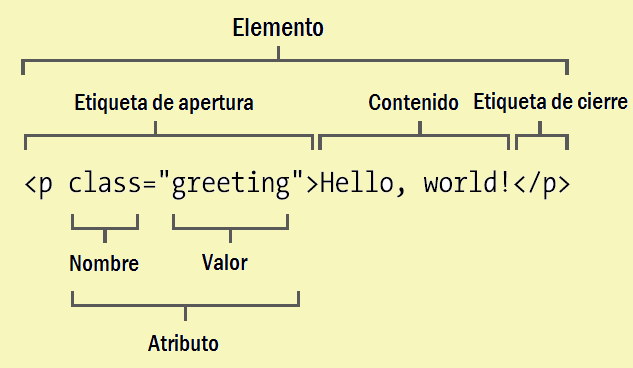
\includegraphics[scale=0.50]{elemento-HTML.png}
    \caption{Partes de un elemento HTML}
\end{figure}

\section{Herramientas de Edición}
Para trabajar con XML es necesario, por un lado, editar los documentos, y por otro procesarlos. Por ello, necesitaremos dos tipos de herramientas para trabajar con él, estas son:

\begin{itemize}
    \item \textbf{Editores XML}

    Una característica de los lenguajes de marcas es que se basan en la utilización de ficheros de \textbf{\gls{texto plano}}, por lo que basta con usar cualquier editor de texto para construir un documento XML.

    Aunque podemos usar cualquier editor, cuando elaboramos documentos XML complejos es conveniente usar
    algún software de edición XML. Estos nos ayudan a crear estructuras y etiquetas de los elementos usados en XML, resaltan las etiquetas para diferenciarlas más cómodamente y ademas incluyen ayudas para la creación de otros elementos como DTD, hojas de estilo CSS o XLS,.. El W3C ha desarrollado un editor HTML, XHTML, CSS y XML gratuito llamado Amaya, pero existen otros muchos gratuitos como: Notepad++, VSCode, Sublime Text, Netbeans,..etc

    \item \textbf{Procesadores XML}

    Para interpretar un documento XML puede usarse cualquier navegador. Los procesadores XML permiten visualizar los documentos XML y acceder a su contenido y estructura. Un \textbf{procesador} es un conjunto de módulos de software entre los que se encuentra un \textbf{parser}, que comprueba que el documento cumple las normas establecidas para que pueda abrirse. Estás normas pueden corresponderse a las necesarias para trabajar con documentos de tipo válido o solo exigir que el documento este bien formado. A los primeros se le conocen como \textbf{procesadores validadores} y a los segundos como \textbf{procesadores no validadores}.

    Para publicar documentos XML en internet se usan \textbf{procesadores XSLT}, que permiten generar archivos HTML a partir de XML.

    Puesto que XML se usa para el intercambio de archivos entre aplicaciones, hay que recurrir a motores independientes como <<XML para Java>> de IBM, JAXP de Sun, etc
\end{itemize}

\section{XML}
\textbf{XML}, que significa \textit{eXtensible Markup Language}, es un lenguaje que permite definir lenguajes de marcas desarrollado por el W3C y utilizado para almacenar datos de forma legible. Proviene del lenguaje SGML y permite definir la gramática de lenguajes específicos para estructurar documentos. \cite{xml}

Su importancia radica en que permite \textbf{compartir datos} entre diferentes equipos y aplicaciones de forma \textbf{segura}, \textbf{fiable} y \textbf{sencilla}. El hecho de que diferentes equipos y aplicaciones puedan leer y generar archivos en este formato lo convierte en una herramienta muy útil para el envío de información a través de la Web. Aunque a veces suele confundirse con HTML, podemos decir que HTML esta diseñado para mostrar datos en nuestras pantallas mientras que XML esta diseñado para almacenar y compartir esos datos.

El XML ahorra tiempos de desarrollo y proporciona ventajas, dotando a webs y aplicaciones de un método muy potente para almacenar y compartir información. Por ello, se ha convertido en un formato universal usado por todo tipo de sistemas operativos y dispositivos.

\subsection{Estructura y Sintaxis}
Un documento XML es un documento de de texto, con la \textbf{extensión .xml}, compuesto de un \textbf{conjunto de etiquetas}, \textbf{estructuradas en árbol}, que describen la organización del documento y que es interpretado por un navegador Web.

La \textbf{características básicas} de XML son las siguientes:

\begin{itemize}
    \item Es directamente \textbf{compatible} con protocolos usados en en la Web como \textbf{HTTP} y \textbf{URL}.
    \item Todo documento que verifique las reglas de XML esta \textbf{conforme con SGML}.
    \item \textbf{No se requieren conocimientos de programación} para realizar tareas sencillas en XML.
    \item Los documentos XML son\textbf{ fáciles de crear}.
    \item \textbf{La difusión} de documentos XML \textbf{está asegurada}, ya que cualquier procesador de XML puede leer documentos XML.
    \item El marcado de XML es \textbf{legible para los humanos}.
    \item El diseño de XML es \textbf{formal y conciso}.
    \item XML es \textbf{extensible}, \textbf{adaptable} y \textbf{aplicable} a una gran variedad de situaciones.
    \item XML es \textbf{orientado a objetos}
    \item Todo documento XML se \textbf{compone} de \textbf{datos de marcado} y \textbf{datos carácter} entremezclados.
\end{itemize}

El \textbf{proceso de creación} de un documento pasa por varias etapas en las que el éxito de cada una de ellas se basa en la calidad de la anterior. Estas etapas son:

\begin{enumerate}
    \item Especificación de requisitos.
    \item Diseño de etiquetas.
    \item Marcado de los documentos.
\end{enumerate}

El \textbf{marcado} son etiquetas que se añaden para estructurar los documentos y permitir a los ordenadores interpretar los textos. Los \textbf{datos carácter} son los que componen la verdad información del documento.

Los documentos XML también pueden \textbf{contener comentarios}, que son interpretados por el intérprete XML y que comienzan con la cadena \textit{<!--} y finalizan con \textit{-->}. Pueden estar en cualquier posición del documento salvo en:

\begin{itemize}
    \item El prólogo
    \item Dentro de una etiqueta
\end{itemize}

Los XML están \textbf{formados} por dos partes, \textbf{el prólogo} y \textbf{el ejemplar}, los cuales veremos a continuación.

\subsection{El Prólogo}
El prólogo es la primera parte que nos encontramos en cualquier documento XML y siempre debe preceder al ejemplar del documento. Éste se divide en dos partes, la \textbf{declaración XML} y la \textbf{declaración de la codificación} empleada, los cuales explicamos a continuación.

\begin{enumerate}
    \item\textbf{La declaración XML}: es la primera linea del documento, de no ser así, se genera un error que impide que el documento sea procesado. En caso de que sea opcional, se permite el procesamiento de documentos HTML y SGML como si fueran documentos XML, si es obligatoria, estos deberán incluir la declaración de la versión XML. Esta declaración permite indicar de forma explicita que el documento es de tipo XML.

    El prologó puede tener \textbf{tres funciones}:

    \begin{enumerate}
        \item \textbf{Declaración de la versión} utilizada de XML:
        \begin{tcolorbox}[sharp corners, colback=yellow!40, colframe=white!20]
             \begin{verbatim}               <?xml version= “1.0”?>\end{verbatim}
         \end{tcolorbox}

         \item \textbf{Declaración de la codificación empleada}:
         \begin{tcolorbox}[sharp corners, colback=yellow!40, colframe=white!20]
          \begin{verbatim}     <?xml version= “1.0” encoding=”iso-8859-1” ?>\end{verbatim}
        \end{tcolorbox}

         En este caso se usa el código código iso-8859-1 (Latin-1) que permite el uso de tildes o caracteres como la <<ñ>>. Otro de los códigos a tener en cuenta es \textbf{\gls{UTF-8}} (\textbf{\gls{unicode}}). Esta codificación soporta más caracteres que iso-8859-1 y permite que estos se visualicen correctamente en más sistemas. Es la \textbf{codificación estándar} recomendada para todos los documentos y la usaremos siempre, salvo que por algún motivo no pueda ser empleada.

         Para consultar más información sobre codificación de caracteres en sistemas informáticos y cuales son los más empleados podemos visitar  \href{https://en.wikipedia.org/wiki/Character_encoding}{página de Wikipedia} sobre codificación de caracteres.

         \item \textbf{Declaración de autonomía del documento}:

         Indica si el documento necesita de otro para su interpretación. Para declararlo, hay que definir el prólogo completo:
         \begin{tcolorbox}[sharp corners, colback=yellow!40, colframe=white!20]
             \small
             \begin{verbatim}<?xml version= “1.0” encoding=”iso-8859-1” standalone=”yes” ?>\end{verbatim}
         \end{tcolorbox}

         La opción \textit{standalone} indica al procesador XML si un documento es independiente (\textit{standalone="yes"}), o si depende de un documento externo, como declaraciones de marcas externas o una DTD externa (\textit{standalone="no"}). Por defecto el documento se considera independiente.
    \end{enumerate}

    \item \textbf{La declaración del tipo de documento}:

    Esta declaración define el tipo de documento que estamos creando para que sea procesado correctamente. Toda declaración de tipo de documento comienza con la cadena:

    \begin{tcolorbox}[sharp corners, colback=yellow!40, colframe=white!20]
        \begin{verbatim}                 <!DOCTYPE Nombre_tipo ...>\end{verbatim}
    \end{tcolorbox}
\end{enumerate}

\subsection{El Ejemplar}
Es la parte más importante de un documento XML ya que contiene los \textbf{datos reales} del documento. Es el \textbf{elemento raíz} de un documento XML y este se nombrará igual que la declaración del tipo de documento (\textit{!DOCTYPE}). Suele estar compuesto de \textbf{elementos anidados}.

En el siguiente ejemplo, el ejemplar es el elemento \textit{<libro>}, que a su vez esta compuesto de los elementos \textit{<titulo>}, \textit{<autoria>}, \textit{<editorial>}, \textit{<isbn>}, \textit{<edicion>} y \textit{<paginas>}.

\begin{figure}[h]
    \begin{tcolorbox}[sharp corners, colback=yellow!30, colframe=white!20]
        \scriptsize
        \begin{verbatim}
      <?xml version="1.0" encoding="utf-8" standalone="yes"?>
      <!DOCTYPE libro>

      <libro>
        <titulo>XML práctico</titulo>
        <autoria>
            <autor>Sebastien Lecomte</autor>
            <autor>Thierry Boulanger</autor>
        </autoria>
        <editorial>Ediciones Eni</editorial>
        <isbn>978-2-7460-4958-1</isbn>
        <edicion>1</edicion>
        <paginas>347</paginas>
      </libro>
        \end{verbatim}
    \end{tcolorbox}
    \caption{Ejemplo del \textit{ejemplar} en un documento XML}
\end{figure}

Es recomendable \textbf{establecer un criterio} y mantenerlo durante todo el documento, por ejemplo, que las etiquetas vayan escritas \textbf{siempre en minúsculas}.

Por otro lado, es conveniente anidar los elementos para una visualización óptima del documento, esto se hará \textbf{indentando} o \textbf{tabulando} el código. A continuación se muestran dos figuras, una sin indentación (errónea) y otra con indentación (correcta).

\begin{figure}[h]
    \begin{tcolorbox}[sharp corners, colback=yellow!30, colframe=white!20]
        \scriptsize
        \begin{verbatim}
        <?xml version="1.0" encoding="utf-8" standalone="yes"?>
        <!DOCTYPE libro>

        <libro>
        <titulo>XML práctico</titulo>
        <autoria>
        <autor>Sebastien Lecomte</autor>
        <autor>Thierry Boulanger</autor>
        </autoria>
        <editorial>Ediciones Eni</editorial>
        <isbn>978-2-7460-4958-1</isbn>
        </libro>
        \end{verbatim}
    \end{tcolorbox}
    \caption{Código XML sin indentación (incorrecto)}
\end{figure}

\begin{figure}[h]
    \begin{tcolorbox}[sharp corners, colback=yellow!30, colframe=white!20]
        \scriptsize
        \begin{verbatim}
        <?xml version="1.0" encoding="utf-8" standalone="yes"?>
        <!DOCTYPE libro>

        <libro>
            <titulo>XML práctico</titulo>
            <autoria>
                <autor>Sebastien Lecomte</autor>
                <autor>Thierry Boulanger</autor>
            </autoria>
            <editorial>Ediciones Eni</editorial>
            <isbn>978-2-7460-4958-1</isbn>
        </libro>
        \end{verbatim}
    \end{tcolorbox}
    \caption{Código XML con indentación (correcto)}
\end{figure}

Como podemos observar, en la segunda figura se reconoce más fácilmente la estructura del documento y se facilita la lectura de este.

Por último, es recomendable \textbf{anidar grupos de datos relacionados}, como se ha hecho en el ejemplo anterior con los elementos \textit{<autor>} dentro del elemento \textit{<autoria}, ya que el documento que \textbf{mas limpio} y \textbf{ordenado}.

\subsubsection{Elementos}
\textbf{Todos los datos} de un documento XML deben \textbf{pertenecer} a un \textbf{elemento del mismo}.

Los elementos son los diferentes \textbf{bloques de información} que permiten definir la \textbf{estructura} del documento XML. Estos está delimitados por una \textbf{etiqueta de apertura} y una \textbf{etiqueta de cierre}. Pueden estar \textbf{compuestos} por \textbf{otros elementos}.

Los \textbf{nombres} de las etiquetas deben ser \textbf{autodescriptivos}, es decir, que ilustren su contenido. Por ejemplo, si estamos con datos relativo a un libro, una etiqueta no debería ser \textit{<caracteristicas>}, ya que es demasiado ambiguo, deberíamos utilizar nombres como \textit{<titulo>}, \textit{<isbn}, etc...

La \textbf{formación de elementos} debe cumplir ciertas \textbf{normas} para que queden bien definidos y que el documento XML al que pertenecen pueda ser procesado sin generar ningún error fatal. Estas normas son las siguientes:

\begin{itemize}
    \item En todo documento XML debe existir \textbf{un documento raíz} y \textbf{solo uno}.
    \item \textbf{Todos} los elementos tienen una \textbf{etiqueta de inicio} y \textbf{otra de cierre}. En caso de que en el documento existan \textbf{elementos vacíos}, se pueden sustituir las etiquetas de apertura y cierre por una de elemento vacío. Esta se construye como una etiqueta de inicio pero añadiendo \textbf{/}, es decir, \textit{<elemento/>} en vez de \textit{<elemento>}. Esta considerada una etiqueta de apertura y cierre.
    \item Al anidar hay que tener en cuenta que \textbf{no puede cerrarse} ningún\textbf{ elemento} que \textbf{contenga otro elemento} que aún \textbf{no se haya cerrado}.
    \item Los \textbf{nombres} de las \textbf{etiquetas de apertura y cierre} deben ser \textbf{idénticos}, respetando las mayúsculas y minúsculas. Pueden ser cualquier cadena alfanumérica que no contenga espacios ni tildes, y que no comience por dos puntos (\textbf{:}), ni por la cadena \textbf{xml}.
    \item El contenido de los elementos \textbf{no puede contener} la cadena <<\textbf{\textit{]]>}}>>, por compatibilidad con SGML. Además, no se pueden utilizar los caracteres \textbf{mayor que} (\textbf{>}), \textbf{menor que} (\textbf{<}), \textbf{ampersand} (\textbf{\&}), \textbf{dobles comillas} (\textbf{"}) y \textbf{apostrofe} (\textbf{`}).

    En caso de tener que utilizar alguno de estos caracteres, se deben sustituir por las siguientes cadenas:

    \begin{table}[ht]
        \centering
        {\renewcommand{\arraystretch}{1.5}
            \begin{tabular}{ |l|l| }
                \hline
                \multicolumn{1}{|c|}{\textbf{Caracteres}} & \multicolumn{1}{|c|}{\textbf{Cadena}} \\ \hline
                \multicolumn{1}{|c|}{>} & \multicolumn{1}{|c|}{\&gt;} \\ \hline
                \multicolumn{1}{|c|}{<} & \multicolumn{1}{|c|}{<\&lt;} \\ \hline
                \multicolumn{1}{|c|}{\&} & \multicolumn{1}{|c|}{\&amp;} \\ \hline
        \end{tabular}}
         \quad
        {\renewcommand{\arraystretch}{1.5}
            \begin{tabular}{ |l|l| }
                \hline
                \multicolumn{1}{|c|}{\textbf{Caracteres}} & \multicolumn{1}{|c|}{\textbf{Cadena}} \\ \hline
                \multicolumn{1}{|c|}{"} & \multicolumn{1}{|c|}{\&quot;} \\ \hline
                \multicolumn{1}{|c|}{'} & \multicolumn{1}{|c|}{\&apos;} \\ \hline
                \multicolumn{1}{|c}{}& \\ \hline
        \end{tabular}}
     \end{table}

     \item Para \textbf{utilizar caracteres especiales}, como £, ©, ®,... hay que usar las expresiones \textit{\textbf{\&\#D;}} o \textit{\textbf{\&\#H;}}, donde D y H se corresponden con el número decimal o hexadecimal, respectivamente, correspondiente al carácter que se quiere representar en código \textbf{UNICODE}.

     En los siguientes enlaces puedes consultar tanto los códigos ASCII y su equivalente en HTML, como el código correspondiente a cada carácter en UNICODE.

     \begin{itemize}
         \item ASCII - \url{https://www.asciitable.com/}
         \item UTF-8 - \url{https://www.charset.org/utf-8}
     \end{itemize}
\end{itemize}

\subsubsection{Atributos}
Las etiquetas pueden tener \textbf{atributos}, que \textbf{permiten definir propiedades} a los elementos de un documento. Los atributos, a diferencia de los elementos, no puede organizarse en ninguna jerarquía	o estructura de árbol, no pueden contener ningún otro elemento, no pueden contener valores múltiples y no reflejan ninguna estructura lógica. En definitiva, los atributos \textbf{no se podrán extender fácilmente} en futuros cambios.

Un elemento puede tener varios atributos, pero ninguno de estos puede estar vacío. Los atributos se codifican de la siguiente forma:

\begin{tcolorbox}[sharp corners, colback=yellow!40, colframe=white!20]
    \begin{verbatim}        <etiqueta atributo="valor_atributo"></etiqueta>\end{verbatim}
\end{tcolorbox}

No debe usarse un atributo para almacenar información susceptible de ser dividida, sino para proporcionar información adicional sobre el elemento. A continuación vamos a ver un ejemplo de la utilización de atributos en un documento XML.

\begin{figure}[h]
    \begin{tcolorbox}[sharp corners, colback=yellow!30, colframe=white!20]
        \scriptsize
        \begin{verbatim}
       <?xml version="1.0" encoding="utf-8" standalone="yes"?>
       <centro_educativo>
           <alumno sexo="Varón" fecha_nacimiento="05/06/1990">
               <nombre>Pablo</nombre>
               <apellido>Pérez</apellido>
               <telefono tipo="Móvil">666666666</telefono>
               <direccion tipo="Calle">Policar, 34</direccion>
           </alumno>
        </centro_educativo>
        \end{verbatim}
    \end{tcolorbox}
    \caption{Uso de atributos en documentos XML}
\end{figure}

Por norma general, intentaremos \textbf{evitar el uso} de atributos o procurar \textbf{no abusar de ellos}. Normalmente \textbf{los usaremos} para \textbf{metadatos} o información que no sea relevante para los datos. Se puede ver como una manera de incorporar características o propiedades a los elementos, como en el siguientes ejemplo: \textit{<perro raza=``Pastor''>Lolo</perro>}. También se suelen para especificar unidades de medida y similares: \textit{altura unidad\_altura=``cm''>178</altura>}. Hay que destacar que toda la información que se almacena en atributos se podría almacenar igualmente en elementos.

Lo que si es recomendable es que \textbf{una vez elegido un estilo}, mantenerlo dentro de todo el documento XML, teniendo en cuenta que los \textbf{nombres de los atributos} tienen que cumplir las \textbf{mismas normas} que los \textbf{elementos}, y no pueden contener el carácter menor que ``<''.

\section{Documentos XML bien formados}
Los documentos XML deben de estar \textbf{bien formados}, es decir, ser documentos \textbf{válidos}.

Los \textbf{documentos bien formados} son aquellos que cumplen las reglas sintácticas de creación de documentos XML ya mencionados en los puntos anteriores, como por ejemplo, que usan caracteres válidos para la creación de nombres de etiquetas o atributos, que las etiquetas estén cerradas correctamente, etc...

Los \textbf{documentos válidos} son aquellos que, ademas de estar bien formados, cumplen los requisitos de una definición de estructura (DTD, Schema,..), que veremos en la siguientes unidad.

Por lo tanto, para que un documento esté bien formado, debe \textbf{verificar} las \textbf{reglas sintácticas} que define la recomendación de la W3C para el \textbf{estándar XML}. Estas normas básicas se pueden resumir en las siguientes:

\begin{itemize}
    \item El documento ha de tener \textbf{definido} una \textbf{declaración XML} en el prólogo:

    \begin{tcolorbox}[sharp corners, colback=yellow!40, colframe=white!20]
        \begin{verbatim}  <?xml version="1.0" encoding="UTF-8" standalone="yes" ?>\end{verbatim}
    \end{tcolorbox}

    Hay que tener en cuenta que aunque es posible omitir el prólogo, hay navegadores que nos pueden devolver un error al procesar el documento, por lo que siempre hay que incluirlo para evitar problemas. En caso de omitirlo, los valores por defecto son los mostrados encima de este párrafo.

    \item Existe un \textbf{único elemento raíz} por cada documento: es un solo elemento en el que todos los demás contenidos y elementos se encuentran anidados.
    \item Los elementos se organizan entre sí en un \textbf{estructura jerárquica} y \textbf{no se permite} el \textbf{solapamiento} de éstos.
    \item Hay que \textbf{cumplir reglas sintácticas} a la hora de definir el nombre de elementos y atributos. Estas normas se pueden resumir en:
    \begin{itemize}
        \item El \textbf{nombre de elementos} puede contener como \textbf{primer carácter} los siguientes: \textit{[A-Z]},  \textit{[a-z]} y \textit{``\_''}. Para el resto de caracteres, ademas de estos, se pueden emplear: \textit{[0-9]}, \textit{``-''} y \textit{``.''}.
        \item Las \textbf{etiquetas de apertura y cierre} deben ser \textbf{idénticas}, teniendo en cuenta que XML es sensible a mayúsculas y minúsculas.
        \item Los \textbf{valores de los atributos} se escribirán siempre entre \textbf{comillas dobles o simples}. Si quisiéramos usar alguno de estos caracteres dentro del nombre usaríamos \&quot; (") y \&apos; ('). También hay que tener en cuenta que hay nombres reservados para el uso del lenguaje.
        \item \textbf{Los comentarios} en XML se escriben así: \textit{ <!-- Comentario -->}
    \end{itemize}
\end{itemize}

\subsection{Espacios de Nombres}
Los \textbf{espacios de nombres} permiten definir la pertenencia de los elementos y nombres a un contexto de vocabulario XML. De esta forma se resuelven las ambigüedades que se pueden producir al juntar dos documentos donde os autores han usado nombres similares para diferentes elementos.

Los espacios de nombres, también conocidos como \textbf{XML namespaces}, permiten dar nombre único a un elemento, indexándolo según un nombre de vocabulario adecuado. Además, están asociados a una \textbf{\gls{URI}}.

En el documento, las etiquetas ambiguas se sustituyen por otras con el nombre precedido de un \textbf{prefijo}, que determina el contexto al que pertenece dicho nombre:

\begin{tcolorbox}[sharp corners, colback=yellow!40, colframe=white!20]
    \begin{verbatim}       <prefijo:nombre_etiqueta></prefijo:nombre_etiqueta>\end{verbatim}
\end{tcolorbox}

Esta etiqueta de denomina \textbf{nombre cualificado}. Al definir el prefijo hay que tener en cuenta que no se pueden usar espacios ni caracteres especiales y que no puede comenzar por un dígito.

Antes de poder usar el espacio de nombres hay que declararlo, es decir, asociar un índice con la URI asignada al espacio de nombres, mediante un atributo \textbf{xmlns}. Esto se hace entre el prólogo y el ejemplar y tiene la siguientes sintaxis:

\begin{tcolorbox}[sharp corners, colback=yellow!40, colframe=white!20]
    \begin{verbatim}   <conexion>://<direccionservidor>/<apartado1>/<apartado2>/...\end{verbatim}
\end{tcolorbox}

Si queremos consultar más información acerca de los espacios de nombres, podemos consultar el estándar en la \href{https://www.w3.org/TR/REC-xml-names/}{recomendación en XML de la W3C}.

\section{Sistemas de Gestión Empresarial}










% Glossary

\glsaddall
\printglossaries

% Bibliography

\newpage
\addcontentsline{toc}{chapter}{Bibliografía}
\bibliography{citas}
\bibliographystyle{unsrt}

\end{document}